% FoodLink -- Activity Diagram: surplus-food donation lifecycle
% (mid-term report copy)
%
% Every decision is a branch the server actually takes. Sources:
%   models.ALLOWED_TRANSITIONS, routers/donations.TRANSITION_ROLES,
%   routers/donations.create_donation / update_status / _record / _claim_pickup,
%   ratelimit.check_donation_creation, matching.score_pair (eligibility gates),
%   routers/admin.expire_overdue.
% Corrected, report-specific redraw of
% `docs/uml/diagrams/02-activity-donation-lifecycle.puml`, which predates the
% overdue-acceptance refusal (D-50), the conditional status write (D-55), the
% coarse pickup area (D-57) and the donor cancellation window (D-58).
% Compile with: pdflatex activity-diagram.tex
\documentclass[border=3pt]{standalone}
\usepackage[T1]{fontenc}
\usepackage{lmodern}
\usepackage{tikz}
\usetikzlibrary{shapes.geometric,shapes.symbols,arrows.meta,calc,
  decorations.pathmorphing,backgrounds}

\begin{document}
\hyphenpenalty=10000
\exhyphenpenalty=10000
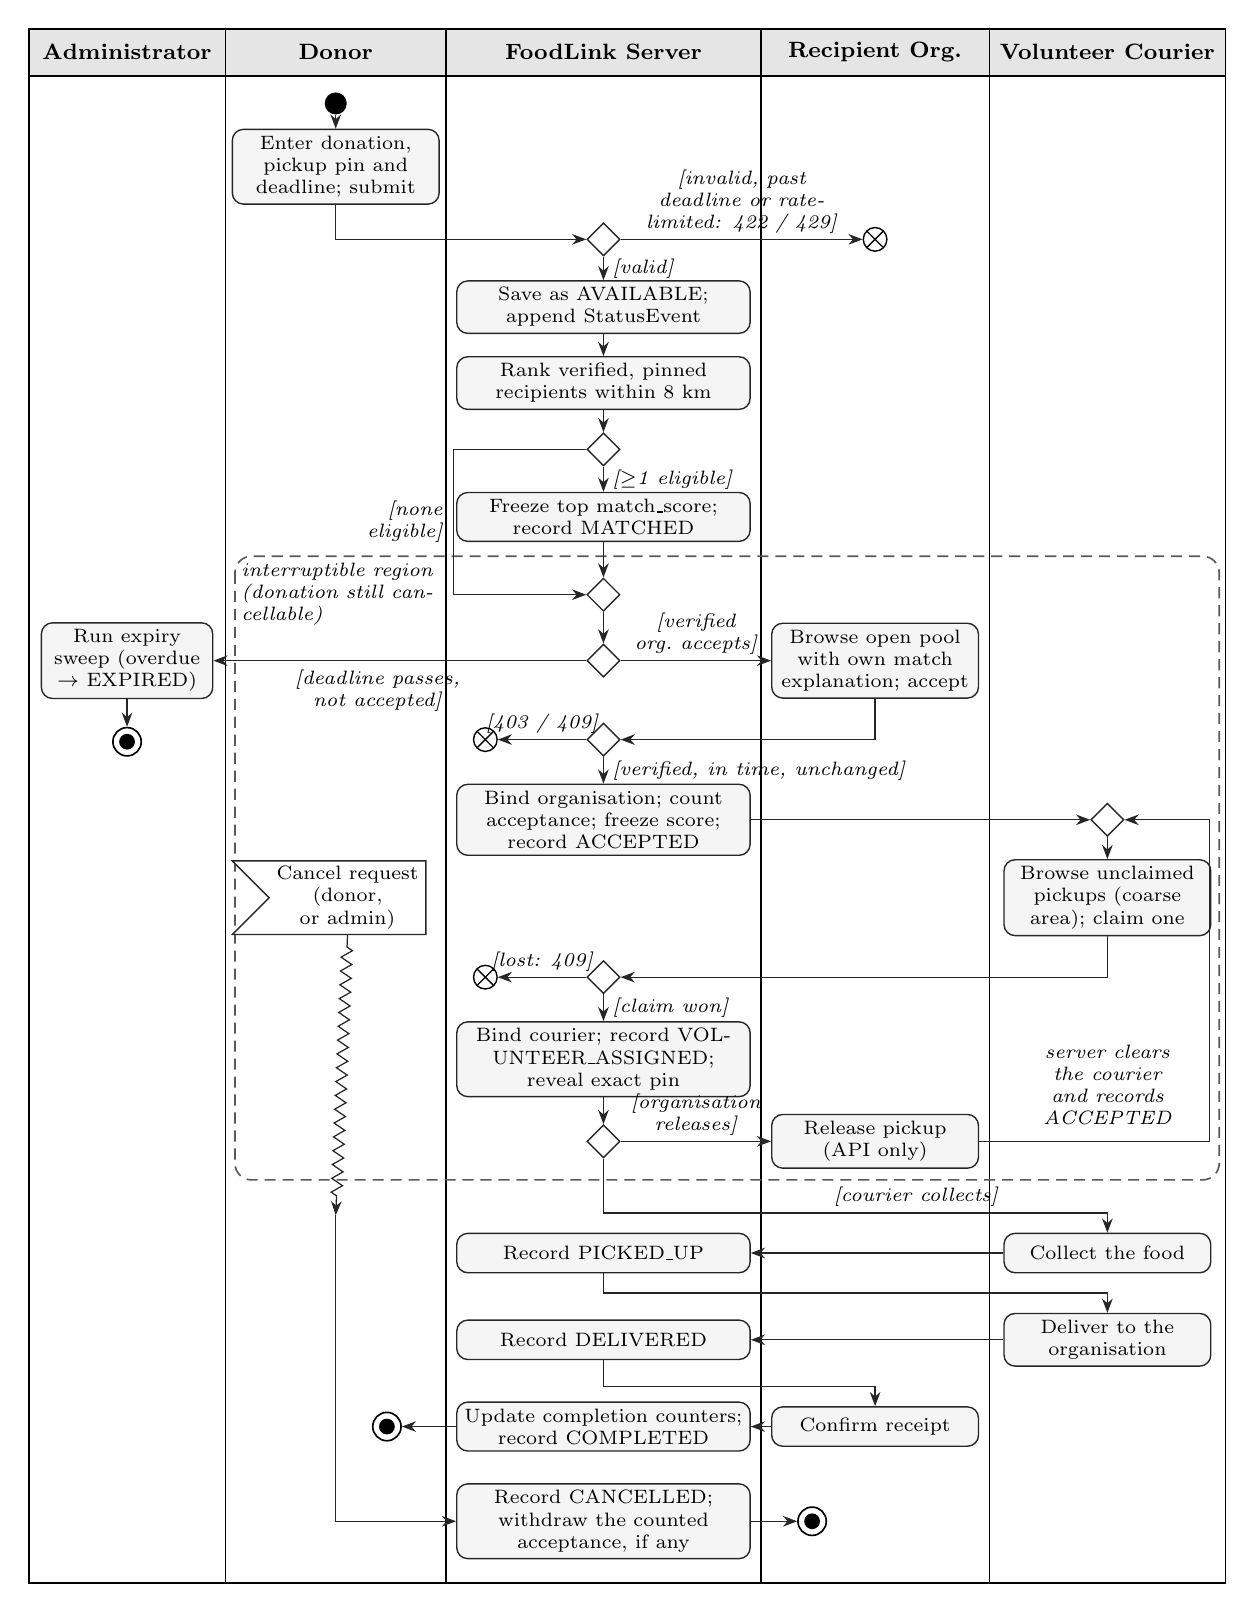
\begin{tikzpicture}[
    font=\scriptsize,
    act/.style={rectangle, rounded corners=4pt, draw=black!85, fill=black!4,
      line width=0.5pt, align=center, inner xsep=2.5pt, inner ysep=2.4pt,
      minimum height=0.5cm},
    srv/.style={act, text width=3.55cm},
    lane/.style={act, text width=2.45cm},
    adm/.style={act, text width=2.0cm},
    dec/.style={diamond, draw=black!85, fill=white, line width=0.5pt,
      minimum size=0.42cm, inner sep=0pt},
    start/.style={circle, fill=black, minimum size=0.28cm, inner sep=0pt},
    stop/.style={circle, draw=black, line width=0.6pt, fill=white,
      minimum size=0.36cm, inner sep=0pt},
    ffinal/.style={circle, draw=black, line width=0.5pt, fill=white,
      minimum size=0.3cm, inner sep=0pt,
      path picture={\draw
        ($(path picture bounding box.north west)+(0.05,-0.05)$) --
        ($(path picture bounding box.south east)+(-0.05,0.05)$)
        ($(path picture bounding box.north east)+(-0.05,-0.05)$) --
        ($(path picture bounding box.south west)+(0.05,0.05)$);}},
    event/.style={signal, signal from=west, signal to=nowhere, draw=black!85,
      fill=white, line width=0.5pt, text width=1.85cm, align=center,
      inner xsep=2pt, inner ysep=2pt},
    flow/.style={draw=black!85, line width=0.45pt, -{Stealth[length=1.8mm]}},
    guard/.style={font=\scriptsize\itshape, inner sep=1pt, align=center},
    hdr/.style={font=\footnotesize\bfseries, align=center},
  ]
  \def\AD{1.25}\def\DO{3.9}\def\SV{7.3}\def\RE{10.75}\def\CO{13.7}

  % ======================= posting ============================================
  \node[start] (s0) at (\DO,0.0) {};
  \node[lane, anchor=north] (d1) at (\DO,-0.32)
    {Enter donation, pickup pin and deadline; submit};
  \node[dec, anchor=north] (q1) at ($(\SV,0 |- d1.south)+(0,-0.22)$) {};
  \node[ffinal] (f1) at (\RE,0 |- q1) {};
  \node[srv, anchor=north] (s2) at ($(q1.south)+(0,-0.3)$)
    {Save as AVAILABLE; append StatusEvent};
  \node[srv, anchor=north] (s3) at ($(s2.south)+(0,-0.28)$)
    {Rank verified, pinned recipients within 8 km};
  \node[dec, anchor=north] (q4) at ($(s3.south)+(0,-0.28)$) {};
  \node[srv, anchor=north] (s5) at ($(q4.south)+(0,-0.32)$)
    {Freeze top match\_score; record MATCHED};
  \coordinate (regionTop) at ($(s5.south)+(0,-0.18)$);
  \node[dec, anchor=north] (m1) at ($(s5.south)+(0,-0.45)$) {};

  \draw[flow] (s0) -- (d1);
  \draw[flow] (d1.south) |- (q1.west);
  \draw[flow] (q1.east) -- node[guard, above=1pt, text width=3.1cm]
    {[invalid, past deadline or rate-limited: 422 / 429]} (f1);
  \draw[flow] (q1) -- node[guard, right=2pt] {[valid]} (s2);
  \draw[flow] (s2) -- (s3);
  \draw[flow] (s3) -- (q4);
  \draw[flow] (q4) -- node[guard, right=2pt] {[$\geq$1 eligible]} (s5);
  \draw[flow] (q4.west) -- (5.4,0 |- q4) -- (5.4,0 |- m1) -- (m1.west);
  \node[guard, anchor=east, text width=1.1cm, align=right]
    at ($(5.3,0 |- q4)!0.5!(5.3,0 |- m1)$) {[none eligible]};
  \draw[flow] (s5) -- (m1);

  % ======================= offer, expiry, acceptance ==========================
  \node[dec, anchor=north] (q6) at ($(m1.south)+(0,-0.4)$) {};
  \node[adm] (a1) at (\AD,0 |- q6) {Run expiry sweep (overdue $\to$ EXPIRED)};
  \node[stop, anchor=north] (e1) at ($(a1.south)+(0,-0.35)$) {};
  \node[lane] (r1) at (\RE,0 |- q6)
    {Browse open pool with own match explanation; accept};
  \node[dec, anchor=north] (q7) at ($(\SV,0 |- r1.south)+(0,-0.3)$) {};
  \node[ffinal] (f2) at (5.8,0 |- q7) {};
  \node[srv, anchor=north] (s8) at ($(q7.south)+(0,-0.34)$)
    {Bind organisation; count acceptance; freeze score; record ACCEPTED};

  \draw[flow] (m1) -- (q6);
  \draw[flow] (q6.east) -- node[guard, above=1pt, text width=1.8cm]
    {[verified org.\ accepts]} (r1.west);
  \draw[flow] (q6.west) -- node[guard, below=2pt, pos=0.56, text width=2.4cm]
    {[deadline passes, not accepted]} (a1.east);
  \draw[flow] (a1) -- (e1);
  \draw[flow] (r1.south) |- (q7.east);
  \draw[flow] (q7.west) -- node[guard, above=1pt] {[403 / 409]} (f2);
  \draw[flow] (q7) -- node[guard, right=2pt] {[verified, in time, unchanged]} (s8);

  % ======================= courier claim and release ==========================
  \node[dec] (m2) at (\CO,0 |- s8) {};
  \node[lane, anchor=north] (c1) at ($(m2.south)+(0,-0.28)$)
    {Browse unclaimed pickups (coarse area); claim one};
  \node[dec, anchor=north] (q9) at ($(\SV,0 |- c1.south)+(0,-0.3)$) {};
  \node[ffinal] (f3) at (5.8,0 |- q9) {};
  \node[srv, anchor=north] (s10) at ($(q9.south)+(0,-0.34)$)
    {Bind courier; record VOLUNTEER\_ASSIGNED; reveal exact pin};
  \node[dec, anchor=north] (q11) at ($(s10.south)+(0,-0.34)$) {};
  \node[lane] (r2) at (\RE,0 |- q11) {Release pickup (API only)};
  \coordinate (regionBot) at ($(r2.south)+(0,-0.14)$);

  \draw[flow] (s8.east) -- (m2.west);
  \draw[flow] (m2) -- (c1);
  \draw[flow] (c1.south) |- (q9.east);
  \draw[flow] (q9.west) -- node[guard, above=1pt] {[lost: 409]} (f3);
  \draw[flow] (q9) -- node[guard, right=2pt] {[claim won]} (s10);
  \draw[flow] (s10) -- (q11);
  \draw[flow] (q11.east) -- node[guard, above=1pt, text width=1.7cm]
    {[organisation releases]} (r2.west);
  \draw[flow] (r2.east) -- (15.0,0 |- r2) -- (15.0,0 |- m2) -- (m2.east);
  \node[guard, text width=2.1cm] at ($(\CO,0 |- r2)+(0,0.72)$)
    {server clears the courier and records ACCEPTED};

  % ======================= collection, delivery, confirmation ================
  \coordinate (collectY) at ($(regionBot)+(0,-0.42)$);
  \node[lane, anchor=north] (c2) at ($(\CO,0 |- collectY)+(0,-0.25)$) {Collect the food};
  \node[srv] (s12) at (\SV,0 |- c2) {Record PICKED\_UP};
  \node[lane, anchor=north] (c3) at ($(c2.south)+(0,-0.5)$) {Deliver to the organisation};
  \node[srv] (s13) at (\SV,0 |- c3) {Record DELIVERED};
  \node[lane, anchor=north] (r3) at ($(\RE,0 |- c3.south)+(0,-0.5)$) {Confirm receipt};
  \node[srv] (s14) at (\SV,0 |- r3) {Update completion counters; record COMPLETED};
  \node[stop] (e2) at (4.55,0 |- s14) {};

  \draw[flow] (q11.south) -- (\SV,0 |- collectY) -- node[guard, above=1pt, pos=0.62]
    {[courier collects]} (\CO,0 |- collectY) -- (c2.north);
  \draw[flow] (c2.west) -- (s12.east);
  \draw[flow] (s12.south) -- ($(\SV,0 |- c2.south)+(0,-0.25)$) --
    ($(\CO,0 |- c2.south)+(0,-0.25)$) -- (c3.north);
  \draw[flow] (c3.west) -- (s13.east);
  \draw[flow] (s13.south) -- ($(\SV,0 |- c3.south)+(0,-0.25)$) --
    ($(\RE,0 |- c3.south)+(0,-0.25)$) -- (r3.north);
  \draw[flow] (r3.west) -- (s14.east);
  \draw[flow] (s14.west) -- (e2);

  % ======================= cancellation (interrupting event) ==================
  \node[event] (ev) at ($(\DO,0 |- c1)+(0.15,0)$) {Cancel request (donor, or admin)};
  \node[srv, anchor=north] (h1) at ($(s14.south)+(0,-0.4)$)
    {Record CANCELLED; withdraw the counted acceptance, if any};
  \node[stop] (e3) at (9.95,0 |- h1) {};
  \foreach \n in {e1,e2,e3} \fill (\n.center) circle (0.1cm);
  \coordinate (zzEnd) at ($(\DO,0 |- regionBot)+(0,-0.45)$);
  \draw[flow, decorate, decoration={zigzag, segment length=5pt, amplitude=2pt,
    pre length=0.15cm, post length=0.2cm}] (ev.south) -- (zzEnd);
  \draw[flow] (zzEnd) |- (h1.west);
  \draw[flow] (h1) -- (e3);

  % ======================= swimlanes and region (background) ==================
  \coordinate (laneBot) at ($(h1.south)+(0,-0.3)$);
  \begin{scope}[on background layer]
    \fill[black!10] (0,0.95) rectangle (15.2,0.35);
    \draw[line width=0.7pt] (0,0.95) rectangle (15.2,0 |- laneBot);
    \draw[line width=0.7pt] (0,0.35) -- (15.2,0.35);
    \foreach \x in {2.5,5.3,9.3,12.2}
      \draw[line width=0.5pt] (\x,0.95) -- (\x,0 |- laneBot);
    \draw[black!65, line width=0.6pt, dash pattern=on 4pt off 2.5pt,
      rounded corners=6pt] (2.62,0 |- regionTop) rectangle (15.12,0 |- regionBot);
  \end{scope}
  \node[guard, anchor=north west, text width=2.55cm, align=left]
    at ($(2.66,0 |- regionTop)+(0,-0.04)$)
    {interruptible region (donation still cancellable)};
  \node[hdr] at (\AD,0.65) {Administrator};
  \node[hdr] at (\DO,0.65) {Donor};
  \node[hdr] at (\SV,0.65) {FoodLink Server};
  \node[hdr] at (\RE,0.65) {Recipient Org.};
  \node[hdr] at (\CO,0.65) {Volunteer Courier};
\end{tikzpicture}
\end{document}
